\documentclass{standalone}
\usepackage{picture,color}
\usepackage{graphicx}
\graphicspath{{./Fig_HIPPOCAMPUS_subfigs/}}
\setlength{\unitlength}{1in}
\usepackage{helvet}
\renewcommand{\familydefault}{\sfdefault}
\begin{document}
\begin{picture}(8.8, 5.51)(0,-5.51)

\put(0.1, -5.5){\includegraphics[width=4.2in]{Fig_HIPPOCAMPUS_subfigs/cnmfe_temporal_v2.pdf}}
\put(0.1, -2.58){\Large\textbf{D}}
\put(1.9, -2.5){\large CNMF-E traces}

\put(4.3, -5.5){\includegraphics[width=4.2in]{Fig_HIPPOCAMPUS_subfigs/ica_temporal_v2.pdf}}
\put(4.3, -2.58){\Large\textbf{E}}
\put(6.0, -2.5){\large PCA/ICA traces}

\put(0.3, -2.2){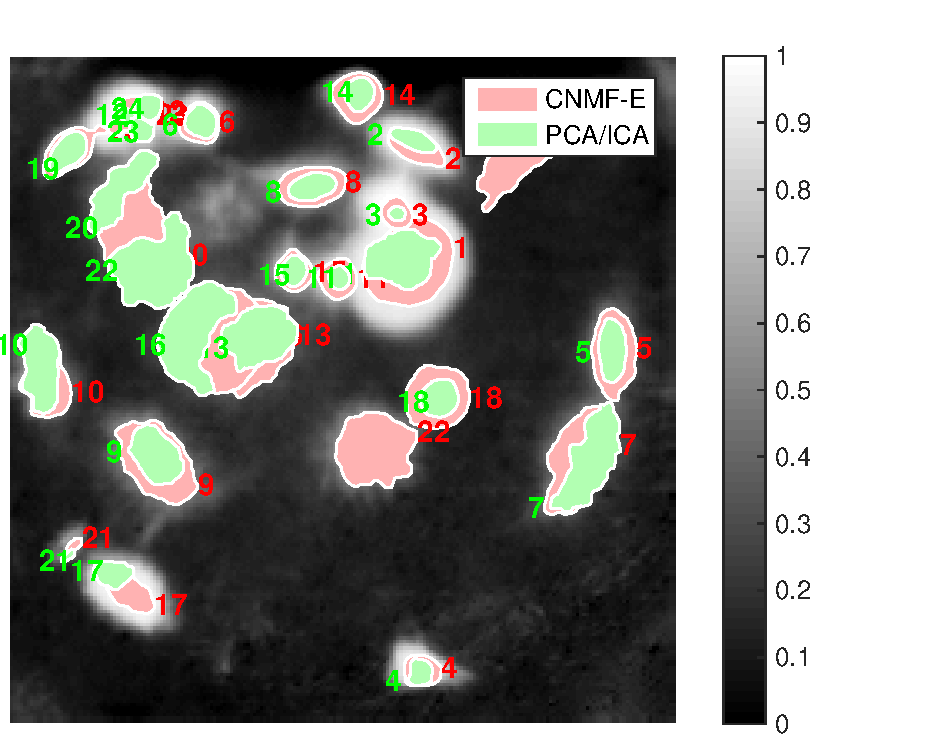
\includegraphics[height=2.0in]{Fig_HIPPOCAMPUS_subfigs/contours.pdf}}
\put(0.1, -0.28){\Large\textbf{A}}
\put(0.55, -0.2){\large Correlation image}


\put(2.59, -2.3){\includegraphics[width=2.9in]{Fig_HIPPOCAMPUS_subfigs/colorbar_cnmfe.png}}
\put(2.65, -1.97){\includegraphics[height=1.6in]{Fig_HIPPOCAMPUS_subfigs/cnmfe_spatial.pdf}}
\put(2.45, -0.28){\Large\textbf{B}}
\put(2.9, -0.2){\large Spatial components, CNMF-E}

\put(5.64, -2.3){\includegraphics[width=2.9in]{Fig_HIPPOCAMPUS_subfigs/colorbar_ica.png}}
\put(5.7, -1.97){\includegraphics[height=1.6in]{Fig_HIPPOCAMPUS_subfigs/ica_spatial.pdf}}
\put(5.5, -0.28){\Large\textbf{C}}
\put(5.95, -0.2){ \large Spatial components, PCA/ICA}


% % traces within an selected ROI 
% \put(2.75, -2.35){\includegraphics[height=2.125in]{Fig_Vessel_subfigs/example_roi_traces.pdf}}
% \put(2.75, -0.25){\large\textbf{B}}
% \put(3.4, -0.16){Fluorescence traces within the ROI}

% % explained variance 
% \put(6.0, -2.32){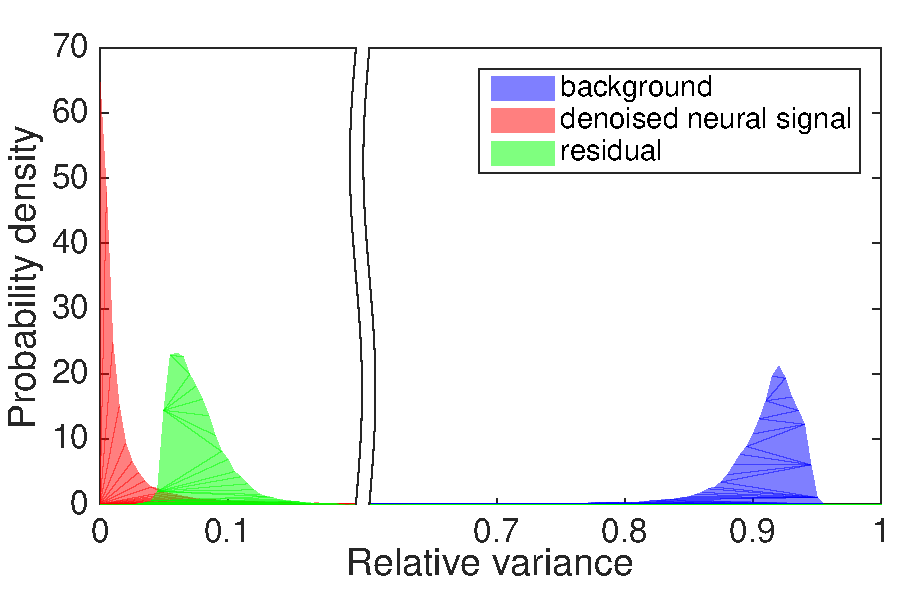
\includegraphics[height=2.25in]{Fig_Vessel_subfigs/variance_explained.pdf}}
% \put(6.0, -0.25){\large\textbf{C}}
% \put(6.95, -0.16){Explained Variance}

% % CNMF-E contours 
% \put(0.05, -4.59){\includegraphics[height=2in]{Fig_Vessel_subfigs/example_contours_cnmfe.pdf}}
% \put(0.1, -2.75){\large\textbf{D}}
% \put(.5, -2.65){CNMF-E contour plot}

% % PCA/ICA contours 
% \put(2.45, -4.59){\includegraphics[height=2in]{Fig_Vessel_subfigs/example_contours_ica.pdf}}
% \put(2.45, -2.75){\large\textbf{E}}
% \put(2.93, -2.65){PCA/ICA contour plot}

% % missed neurons 
% \put(5., -4.52){\includegraphics[height=1.8in]{Fig_Vessel_subfigs/missed_spatial.pdf}}
% \put(4.85, -2.75){\large\textbf{F}}
% \put(5.12, -2.65){Spatial}
% \put(5.75, -4.82){\includegraphics[height=2.1in]{Fig_Vessel_subfigs/missed_temporal.pdf}}
% \put(6.8, -2.65){Temporal components}

% % matched neurons 
% \put(0.25, -6.8){\includegraphics[height=1.8in]{Fig_Vessel_subfigs/match_spatial_cnmfe.pdf}}
% \put(0.1, -5.03){\large\textbf{G}}
% \put(0.31, -4.92){CNMF-E}

% \put(7.9, -7.05){\includegraphics[height=2.1in]{Fig_Vessel_subfigs/snr_pca_ica.pdf}}
% \put(7.95, -5.03){\large\textbf{I}}
% \put(8.6, -4.92){PNR}

% \put(1.9, -7.1){\includegraphics[height=2.1in]{Fig_Vessel_subfigs/matched_temporal.pdf}}
% \put(3.0, -4.92){CNMF-E traces}
% \put(5.85, -4.92){PCA/ICA traces}
% \put(1.9, -5.03){\large\textbf{H}}

% \put(1.01, -6.8){\includegraphics[height=1.8in]{Fig_Vessel_subfigs/match_spatial_ica.pdf}}
% \put(1.08, -4.92){PCA/ICA}

% \put(2.0, -0.9){\Large $=$}

\end{picture}
\end{document}
